\section{Experiment 1: Quadratic Voting, Likert scale surveys and Donation}
\subsection{Methodology} \label{method-1}
The first experument aims to 
answer research questions one and three.
We collected 213 valid submissions %actual 216, screens 3.4K
from Mturk in 2020.
Participants were recruited 
to match the US 2019 census 
on education level and age.
Participants were told that this study
aims to understand their opinions
toward societal causes and 
will be asked to complete a dontaion task.
Participants recieved \$0.75 and \$1.75
according to the groups they are assigned to.
Once participants submitted 
the consent form and demographic survey,
they were equally distributed into seven groups
based on their demographics.

\begin{figure}[htpb]
    \centering
    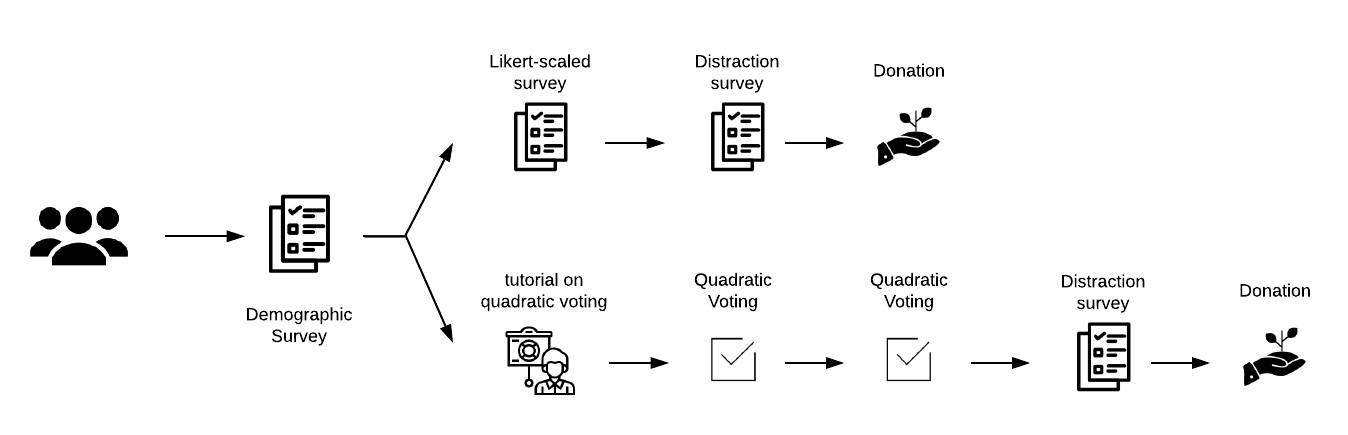
\includegraphics[width=\textwidth, keepaspectratio=true]{content/image/exp1_flow.png}
    \caption{
        Experiment 1 Flow Chart
    }
    \Description[Image describing the flow for experiment 1]{Image describing the flow for experiment 1}
    \label{fig:exp1_image_flow}
\end{figure}

The first group of participants,
know as the Likert group (Upper path in Graph \ref{fig:exp1_image_flow}),
will reveal their opinion
using a Likert scale survey.
The second to seventh group of participants,
the QV group (Lower path in Graph \ref{fig:exp1_image_flow}),
will reveal their preference
by completing two QVs 
with different numbers of voice credits
successively. 
These two voice credits are draw from 
the three possible values: 
$N \times O$, $N^1.5 \times O$, $N^2 \times O$,
where $N$ is the number of options
in the survey and 
$O$ is the number of levels excluding netural
on the likert scale survey. %not sure if this is clear
In our case, with nine options 
and used a five-point Likert scale survey,
the three values would be 
$36$, $108$ and $324$.

% Explain text: On a 5-point Likert scale, user can vote at most 2 levels positive or 2 levels negative (and a neutral). We want to make sure that in a QV, user have enough budget to cast 2 votes either positively or negatively for all options, similar to the Likert survey (so that we are not over limiting their ability to express the same intensity in QV). In QV, 2 votes cost 4 credits. So, the minimum number of total voice credits is 4 * # of options = 4*9 = 36. To test how larger budgets impact people's choices, we set an exponential increase in the total voice credits based on the number of options. In the minimum case, we use (# of option)^1. We scale the budget as (# of option)^1.5 and (# of option)^2 in the second and third budget. Hence, the second budget is 4 * (# of option)^1.5 = 4 * 27 = 108. The third budget is 4 * (# of option)^2 = 4 * 81 = 324.

To ensure evey participant
in the QV group
fully understand how QV works,
they are presented 
with a prerecorded tutorial video
of QV's concept and how to operate the interface.
Participants are granted unlimited time
to interact with the QV interface.
Once participants feel comfortable to mvoe on, 
they will need to correcly answer at least three
of five mutiple choice questions 
on QV and the video,
to continue with the survey.
We also designed 
a distraction surveys
that contains a series of short answer questions
which were also related to societal issues
right after their likert scale survey or QV.
This prevents participants to 
connect their answers to their final donation task.\par

The same prompt were described 
to the participants in the same way
across likert, QV and the donation task
to make them comparable.
We explicitly tell the participants that
there are limited resources in the society,
and ask the participants
``What societal issues need more support?''\par

\subsection{Societal Causes and Charities}
We used the categorization of charity groups on Amazon Smile,
a popular donation website 
that has accumulated over 100 million dollars of donations
as our topics of the societal causes.
The categories are: 
(1) Pets and Animals 
(2) Arts, Culture, Humanities  
(3) Education 
(4) Environment 
(5) Health 
(6) Human Services 
(7) International 
(8) Faith and Spiritual, and
(9) Veteran.
Within each of these categories, 
we select one charity from Amazon Smile
as the representation
of the subject matter used in the donation task.

\subsection{System Design}
The voting system is constructed 
using Python Flask for the back-end, 
Angular for front-end and 
MongoDB for database storage. 
The experiment source code is 
publicly available \footnote{Not yet public} 
and the QV interface is also provided 
as a stand-alone repository \footnote{https://github.com/hank0982/QV-app}.
This system is completely redesigned to ensure
the stability and extensibility
compared to the pre-test system.

% \begin{figure}[htpb]
%     \centering
%     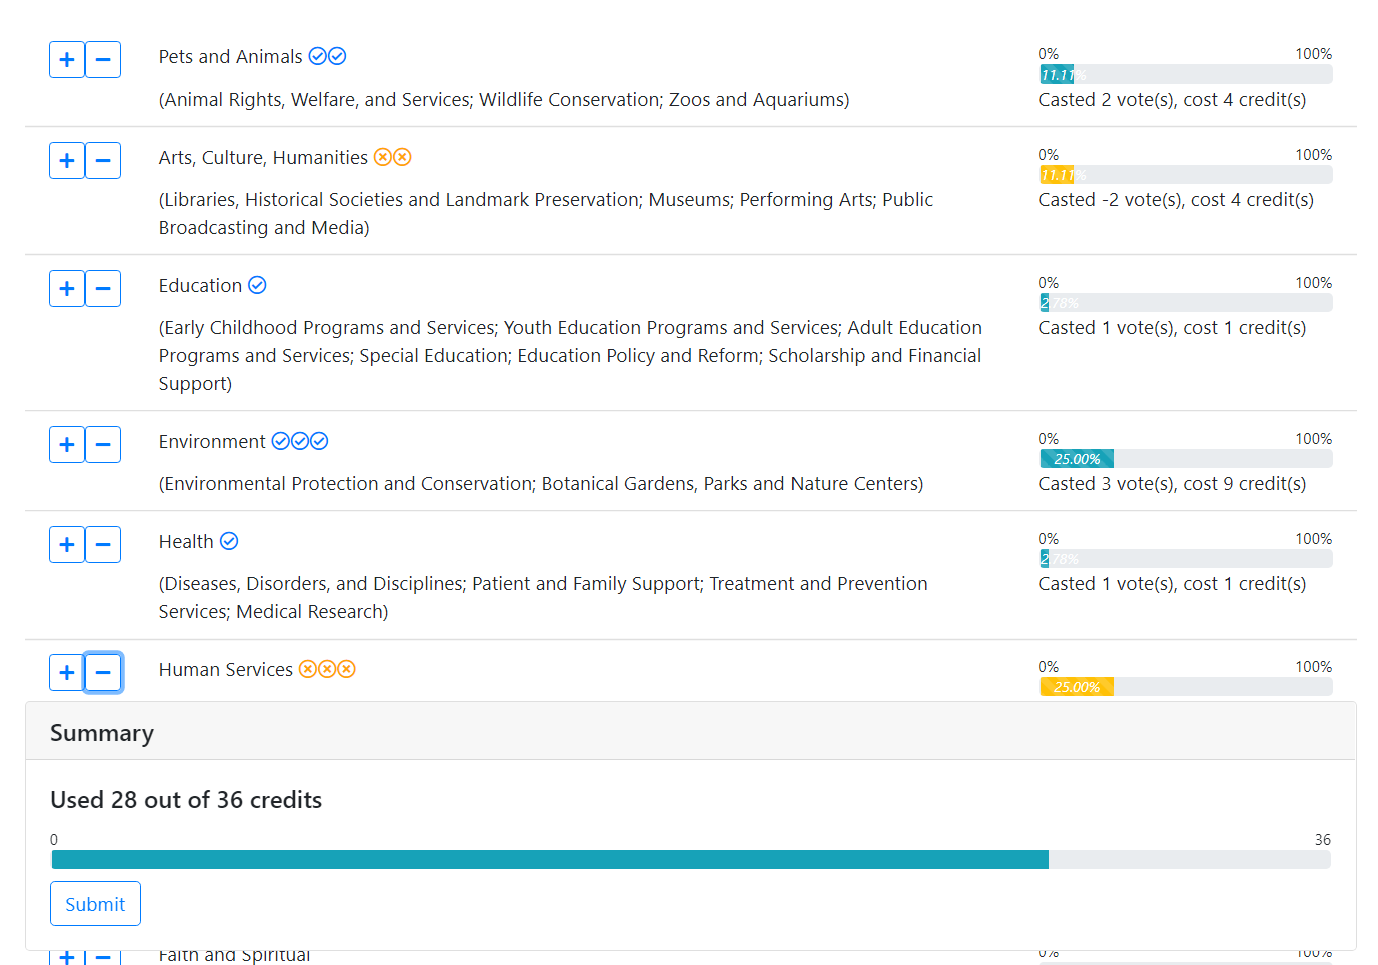
\includegraphics[width=0.7\textwidth, keepaspectratio=true]{resources/qv-donation.png}
%     \caption{
%         QV interface in the new system
%     }
%     \label{fig:qv_donation}
% \end{figure}
% \begin{figure}[htpb]
%     \centering
%     \includegraphics[width=\textwidth, keepaspectratio=true]{resources/donation.jpg}
%     \caption{
%         Donation Interface for experiment one. 
%         Some options were excluded.
%     }
%     \label{fig:donation}
% \end{figure}

The QV interface, 
shown in Figure \ref{fig:qv_donation} 
consists of much more information
to assist the participants.
The summary section 
now floats at the bottom of the page
to ensure visibility
and usability.
Similar in the pretest,
a progress bar will show the number of votes
that the participants cast 
and had not cast.
Beneath the summary bar,
we list a set of options to vote upon.
To the left of the options,
participants vote using the plus and minus buttons.
Buttons are disabled 
if the number of voice credit 
does not permit the next vote.
A bar on the right of the option 
shows the proportion of voice credits used to that option
with text associated with the visual.
The different colors and the icons to the right of each option
exhibits for or again that option.\par

The donation interface is also shown in
Figure \ref{fig:donation}. 
This figure omitted some of the donation options
that were present in the experiment.
The sequence of the donation organizations 
are randomized for each participant
also to ensure ecological validity.
Participants cannot enter value 
that exceeds the 35 dollar amount.
A summary is also displayed 
at the bottom of the page
to assist the participant
at making their decisions.\par